\part{物理损害所致急诊}

\chapter{中 暑}

中暑(heat
illness)是在暑热天气、湿度大和无风的环境条件下,表现以体温调节中枢功能障碍、汗腺功能衰竭和水电解质丧失过多为特征的疾病。重症中暑依其主要发病机制和临床表现不同常分为三型:①热痉挛(heat
cramp);②热衰竭(heat exhaustion);③热(日)射病(heat stroke,sun
stroke)。该三型可顺序发展,也可交叉重叠。热(日)射病是一种致死性疾病,病死率较高,介于20\%~70\%。

\subsection{病因与发病机制}

对高温环境的适应能力不足是致病的主要原因。在大气温度升高(>
32℃)、湿度较大(>
60\%)和无风的环境中,长时间工作或强体力劳动,又无足够的防暑降温措施时,缺乏对高温环境适应者极易发生中暑。此外,在室温较高和通风不良的环境中,年老体弱、肥胖者也易发生中暑。通常,湿热(气温高和湿度大)环境较干热(气温高和辐射强)环境更易发生中暑。老年、体弱、疲劳、肥胖、饮酒、饥饿、失水、失盐、穿着紧身、不透风的衣裤以及发热、甲亢、糖尿病、心血管病、广泛皮肤损害、先天性汗腺缺乏症和应用阿托品或其他抗胆碱能神经药物而影响汗腺分泌等因素,在炎热季节常为中暑的发病诱因。

中暑损伤主要是由于体温过高(>
42℃)对细胞直接损伤作用,引起酶变性、线粒体功能障碍、细胞膜稳定性丧失和有氧代谢途径中断,导致多器官功能障碍或衰竭。

热痉挛的发生机制是高温环境中,人的散热方式主要依赖出汗。一般认为一个工作日的最高生理限度的出汗量为6L,但在高温环境中劳动者的出汗量可在10L以上。汗中含氯化钠约0.3\%~0.5\%。因此大量出汗使水和钠盐过多丢失,使肌肉痉挛,并引起疼痛。

热衰竭的发病机制主要是由于人体对热环境不适应引起周围血管扩张、循环血量不足、发生虚脱;热衰竭亦可伴有过多的出汗、失水和失盐。

热射病的主要发病原因是由于人体受外界环境中热原的作用和体内热量不能通过正常的生理性散热以达到热平衡,致使体内热蓄积,引起体温升高。初起,可通过下视丘体温调节中枢以加快心输出量和呼吸频率,皮肤血管扩张,出汗等提高散热效应。而后,体内热进一步蓄积,体温调节中枢失调,心功能减退,心输出量减少,中心静脉压升高,汗腺功能衰竭,使体内热进一步蓄积,体温骤增。体温达42℃以上可使蛋白质变性,超过50℃数分钟细胞即死亡。

\subsection{诊断}

\subsubsection{临床表现特点}

根据我国《职业性中暑诊断标准》(GB11508-89),可将中暑分为先兆中暑、轻症中暑和重症中暑三级,其临床特点如下。

\hypertarget{text00354.htmlux5cux23CHP15-1-2-1-1}{}
(一) 先兆中暑

在高温环境下工作一定时间后
,出现头昏、头痛、口渴、多汗、全身疲乏、心悸、注意力不集中、动作不协调等症状。体温正常或略有升高。如及时将患者转移到阴凉通风处安静休息,补充水、盐,短时间内即可恢复。

\hypertarget{text00354.htmlux5cux23CHP15-1-2-1-2}{}
(二) 轻症中暑

除上述症状加重外,体温至38℃以上,出现面色潮红,大量出汗,皮肤灼热等表现;或出现面色苍白、皮肤四肢湿冷、血压下降、脉搏增快等虚脱表现。如进行及时有效的处理,常常于数小时内恢复。

\hypertarget{text00354.htmlux5cux23CHP15-1-2-1-3}{}
(三) 重症中暑

包括热痉挛、热衰竭和热射病三型。

\paragraph{热痉挛}

常发生在高温环境中强体力劳动后。由于出汗过多,口渴,大量饮水而盐分补充不足以致血中氯化钠浓度显著下降,而引起四肢阵发性的强直性痉挛,最多见于下肢双侧腓肠肌,常伴有肌肉疼痛、腹绞痛及呃逆。体温大多正常。实验室检查有血钠和氯化物降低,尿肌酸增高。可为热射病的早期表现。

\paragraph{热衰竭}

常发生于老年人、儿童、慢性疾病患者及一时未能适应高温气候及环境者。严重热应激时,由于体液和体钠丢失过多引起循环血容量不足所致。患者先有头痛、头晕、恶心,继而有口渴、胸闷、脸色苍白、冷汗淋漓、脉搏细弱或缓慢、血压偏低。可有晕厥,并有手、足抽搐。体温可轻度升高。重者出现周围循环衰竭。实验室检查有血细胞比容升高、高钠血症、轻度氮质血症和肝功能异常。热衰竭可以是热痉挛和热射病的中介过程,如不治疗可发展成为热射病。

\paragraph{热射病}

是一种致命性急症,典型表现为高热(>
41℃)和意识障碍。根据发病时患者所处的状态和发病机制,临床上分为两种类型:劳力性和非劳力性(或典型性)热射病,前者主要是在高温环境下内源性产热过多;后者主要是在高温环境下体温调节功能障碍引起散热减少。

\hypertarget{text00354.htmlux5cux23CHP15-1-2-1-3-3-1}{}
(1) 劳力性热射病(exertional heatstroke):

多在高温、湿度大和无风天气进行重体力劳动或剧烈体育运动时发病。患者多为平时健康的年轻人,在从事重体力劳动或剧烈运动数小时后发病,约50\%患者大量出汗,心率可达160~180次/分钟,脉压增大。可发生横纹肌溶解、急性肾衰竭、肝衰竭、DIC或MODS,病死率较高。

\hypertarget{text00354.htmlux5cux23CHP15-1-2-1-3-3-2}{}
(2) 非劳力性热射病(nonexertional heatstroke):

在高温环境下,多见于居住拥挤和通风不良的城市的老年体衰居民。其他高危人群包括精神分裂症、帕金森病、慢性酒精中毒及偏瘫或截瘫患者。表现皮肤干热和发红,84\%~100\%病例无汗,直肠温度常>
41℃,最高可达46.5℃。病初表现行为异常或癫痫发作,继而出现谵妄、昏迷,严重者出现低血压、休克、心律失常及心力衰竭、肺水肿及脑水肿等。

实验室检查有血白细胞升高,尿蛋白和管型出现,血尿素氮(BUN)、AST、ALT、LDH、CK增高,血pH降低,血Na\textsuperscript{+}
、K\textsuperscript{+} 降低。心电图检查有心律失常和心肌损害的表现。

\subsubsection{诊断注意事项}

中暑的诊断可根据在高温环境中劳动和生活时出现体温升高、肌肉痉挛和(或)晕厥,并应排除其他疾病后方可诊断。此外,尚必须与其他疾病鉴别。如热射病必须与脑型疟疾、脑炎、脑膜炎、有机磷农药中毒、中毒性肺炎、菌痢等鉴别;热衰竭应与消化道出血或宫外孕、低血糖等鉴别;热痉挛伴腹痛应与各种急腹症鉴别。

\subsection{治疗}

\paragraph{先兆中暑与轻症中暑}

应立即撤离高温环境,在阴凉处安静休息并补充清凉含盐饮料,即可恢复。疑有循环衰竭倾向时,可酌情给葡萄糖盐水静滴。体温升高者及时行物理降温。

\paragraph{热痉挛与热衰竭}

患者应迅速转移到阴凉通风处休息或静卧。口服凉盐水、清凉含盐饮料。静脉补给生理盐水、葡萄糖液和氯化钾。一般患者经治疗后30分钟到数小时内即可恢复。

\paragraph{热射病}

须紧急抢救,降温速度决定预后。应在1小时内使直肠温度降至38.5℃以内。

\hypertarget{text00354.htmlux5cux23CHP15-1-3-3-1}{}
(1) 体外降温:

将患者转移到通风良好的低温环境,脱去衣服,按摩四肢皮肤,使皮肤血管扩张和加速血液循环,促进散热。对无循环虚脱的患者,可用冷水擦浴或将躯体浸入27~30℃水中传导散热降温。对循环虚脱的患者可用蒸发散热降温,如用15℃冷水反复擦拭皮肤或同时应用电风扇或空气调节器。或在头部、腋窝、腹股沟处放置冰袋,并用电扇吹风,加速散热。农村无上述条件时可用井水或泉水擦洗,促进蒸发降温。

\hypertarget{text00354.htmlux5cux23CHP15-1-3-3-2}{}
(2) 体内降温:

体外降温无效者,用冰盐水进行胃或直肠灌洗,也可用20℃或9℃无菌生理盐水进行血液透析或腹膜透析,或将自体血液体外冷却后回输体内降温。

\hypertarget{text00354.htmlux5cux23CHP15-1-3-3-3}{}
(3) 药物降温:

常用氯丙嗪。用法:将氯丙嗪25~50mg稀释在500ml葡萄糖盐水或生理盐水中静滴1~2小时,病情紧急时可用氯丙嗪及异丙嗪各25mg稀释于5\%葡萄糖液100~200ml中,在10~20分钟内静滴完毕。如1小时内体温仍未下降可重复一次。肛温降至约38℃时应暂停,如体温回升可重复运用,有心血管病史慎用。

\hypertarget{text00354.htmlux5cux23CHP15-1-3-3-4}{}
(4) 对症治疗:

保持患者呼吸道通畅,并给予吸氧;烦躁不安或抽搐者,可用地西泮(安定)10mg或苯巴比妥钠0.1~0.2g/次肌注;纠正水、电解质与酸碱平衡失调;应用肾上腺皮质激素对高温引起机体的应激和组织反应以及防治脑水肿、肺水肿均有一定的效果;应用B族维生素和维生素C,以及脑细胞代谢活化剂;防治心、肾、呼吸功能不全,防治感染等。

\protect\hypertarget{text00355.html}{}{}

\hypertarget{text00355.htmlux5cux23CHP15-1-4}{}
参 考 文 献

1. 职业性中暑诊断标准及处理原则 .中国工业医学杂志,1990,3:51

2. 陆再英,钟南山.内科学.第7版.北京:人民卫生出版社,2008:958

\protect\hypertarget{text00356.html}{}{}

\chapter{晕 动 病}

乘车、船或飞机时,因摇摆、颠簸、旋转或加速等刺激,主要使前庭功能紊乱而致的一系列自主神经功能失调症状,称晕动病(motion
sickness)。

\subsection{病因与发病机制}

晕动病的发病机制主要与影响前庭功能有关。前庭器内耳膜迷路的椭圆囊和球囊的囊斑是感受上下、前后和左右的直线运动,三个半规管毛细胞感受旋转运动。当囊斑或毛细胞受到一定量的不正常运动刺激所引起的神经冲动,依次由前庭神经传至前庭神经核,再传至小脑和下丘脑,因而引起一系列以眩晕为主要症状的临床表现。前庭受刺激后影响网状结构,引起血压下降和呕吐。前庭神经核通过内侧纵束纤维至眼肌运动核引起眼球震颤。小脑和下丘脑受神经冲动后引起全身肌肉张力改变。晕动病与视觉可能有一定关系,如当人们凝视快速运动或旋转的物体时也同样可引起本病。小脑受刺激亦可能为本病的发病因素。此外,高温、高湿、通风不良、噪音、特殊气味、情绪紧张、睡眠不足、过度疲劳、饥饿或过饱、身体虚弱、内耳疾病等均易诱发本病。本病的个体易感性变化较大,2~12岁易感性较高。

\subsection{诊断}

本病常在乘车、船、飞机和其他运行数分钟至数小时后发生。初时感觉上腹不适,即有恶心、面色苍白、乏力、心跳加速、出冷汗,旋即有眩晕、精神抑郁、唾液分泌增多和呕吐。可有血压下降、呼吸深而慢、眼球震颤。严重呕吐引起失水和电解质紊乱。症状一般在停止运行或减速后数十分钟和数小时内消失或减轻;亦有持续数天后才逐渐恢复,并伴有精神萎靡、四肢无力。

本病应与内耳眩晕病、前庭神经炎、椎基底动脉供血不足等疾病相鉴别。

\subsection{治疗}

\paragraph{一般处理}

发病时患者宜闭目仰卧,松解领扣、腰带,指压或针刺内关、合谷等穴位有一定效果。坐位时头部紧靠在固定椅背或物体上,避免较大幅度的摇摆。环境要安静,通风良好。有呕吐剧烈、脱水和低血压者,应静脉补充液体和电解质。

\paragraph{药物治疗}

主要应用抗组胺类和抗胆碱能类药物治疗,可单独应用或联合用药。常用药物有:

\hypertarget{text00356.htmlux5cux23CHP15-2-3-2-1}{}
(1) 氢溴酸东莨菪碱(scopolamine hydrobromide):

0.3~0.6mg口服,每日3次。青光眼患者忌用。

\hypertarget{text00356.htmlux5cux23CHP15-2-3-2-2}{}
(2) 茶苯海明(dimenhydrinate,乘晕宁,晕海宁):

为苯海拉明和8-绿茶碱的复合物。25~50mg口服,每日3次。副作用有嗜睡、皮疹等。

\hypertarget{text00356.htmlux5cux23CHP15-2-3-2-3}{}
(3) 倍他司汀(抗眩啶):

4~8mg口服,每日3次。

\hypertarget{text00356.htmlux5cux23CHP15-2-3-2-4}{}
(4) 美可洛嗪(敏可静,meclizine):

为哌嗪类抗组胺药,作用持续12~24小时。25mg口服,每日1~3次。副作用有嗜睡、视力模糊、口干、乏力等。

\hypertarget{text00356.htmlux5cux23CHP15-2-3-2-5}{}
(5) 布可利嗪(buclizine,安其敏):

为哌嗪类抗组胺药。25mg口服,每日3次,副作用有嗜睡、眩晕等。

\hypertarget{text00356.htmlux5cux23CHP15-2-3-2-6}{}
(6) 异丙嗪(promethazine,非那根):

为吩噻嗪类抗组胺药。口服每次12.5~25mg,每日2~3次;肌内注射每次25~50mg。副作用为困倦、嗜睡、口干等。

\hypertarget{text00356.htmlux5cux23CHP15-2-3-2-7}{}
(7) 苯海拉明(diphenhydramine):

为乙醇胺类抗组胺药。口服每次25mg,每日3~4次;肌内注射每次20mg,每日1~2次。副作用有头晕、头痛、嗜睡、口干、恶心、乏力等。

\hypertarget{text00356.htmlux5cux23CHP15-2-3-2-8}{}
(8) 甲氧氯普胺(metoclopramide,胃复安,灭吐灵):

5~10mg口服,每日3次;肌内注射每次10~20mg。

\hypertarget{text00356.htmlux5cux23CHP15-2-3-2-9}{}
(9) 多潘立酮(domperidone,吗丁啉):

口服每次10~20mg,每日3次,饭前服;肌内注射每次10mg。

\hypertarget{text00356.htmlux5cux23CHP15-2-3-2-10}{}
(10) 其他药物:

如氯丙嗪、地西泮(安定)、苯巴比妥等亦可酌情使用。

易患本病的患者,应积极寻找诱发原因,并加以避免。起程前避免饱餐、饮酒和过度疲劳。在旅行途中应闭目静坐,不要观看旅途两旁晃动物体,避免阅读。在旅行前0.5~1小时先服用上述药物一次剂量,可减轻症状或避免发病。

\protect\hypertarget{text00357.html}{}{}

\hypertarget{text00357.htmlux5cux23CHP15-2-4}{}
参 考 文 献

1. 陈灏珠 ,林果为.实用内科学.第13版.北京:人民卫生出版社,2009:881

2. 张文武 .急诊内科学.第2版.北京:人民卫生出版社,2007:1416

\protect\hypertarget{text00358.html}{}{}

\chapter{冷 伤}

冷伤(cold
injury)是机体遭受低温侵袭所引起的局部或全身性损伤,分为非冻结性冷伤和冻结性冷伤(frost
cold
injury)两大类。非冻结性冷伤是人体接触10℃以下、冰点以上的低温,加上潮湿条件所造成的损伤,包括冻疮、“战壕足”、“水浸手、水浸足”等。冻结性冷伤是由冰点以下低温所造成,包括局部冻伤(frostbite)和全身性冷伤。全身性冷伤又称“冻僵”(frozen
rigor,frozen stiff)、意外低体温(accidental
hypothermia),是寒冷环境引起体温过低所导致以神经系统和心血管损伤为主的严重的全身性疾病。

\subsection{病因与发病机制}

正常人体体温的保持依靠神经内分泌的调节,通过体内代谢产热和机体散热(受气候条件等影响)以维持动态平衡,保持相对稳定的水平。任何因素,特别是外界气温的影响,使机体产生的热量不足以代偿丧失的热量,超过机体可调节的限度时,则会发生冷伤。寒冷的程度是造成冷伤的主要原因。但气候条件也会加强低温的致伤作用,潮湿和风都可加速身体的散热;身体暴露于寒冷中的时间越长,发生冷伤的机会越多。任何使局部血液循环发生障碍,热量来源减少的因素,都可促使冷伤的发生。例如,鞋、袜带过紧、长时间静止不动或四肢绑扎止血带等。还有一些降低人体抵抗力的因素,同样也减弱人体对外界温度变化的适应和调节能力,从而在寒冷环境中易发生全身性和局部性冷伤。例如,创伤、休克、过度疲劳、酒醉、营养不良等。由于人体对于低温的耐受力差异很大,因此每个人发生冷伤的程度也不一样,这主要同耐寒锻炼的多少有关,长年居住在寒冷地方的人对于寒冷的适应和耐受能力明显强于处于温暖气候中的人。

非冻结性冷伤是由温度在冰点以上的低温引起,如冻疮、“战壕足”、“水浸手、水浸足”等,其发生机制一般认为低温与潮湿共同作用,使血管长时间处于痉挛状态,从而导致微血管损伤,引起水肿和血栓形成,造成组织损伤、坏死。冻疮(chilblain)是指在温度不低于冰点,但周围环境高湿度的情况下,肢体末梢、耳鼻等处的皮肤轻度冷伤,表现为局部有痒感或胀痛的皮肤紫红色斑、丘疹或结节病变,可伴水肿与水疱。病程中表皮可脱落,出血、糜烂或出现溃疡,最终形成瘢痕或纤维化。“战壕足”过去多发生于战时,是长时间站立在1~10℃的壕沟所引起。“水浸手、水浸足”是指长时间将手足浸入寒冷水中所致的冷伤,较多见于海员、渔民、水田劳作以及施工人员。

冻结性冷伤受伤到复温后的改变可分为以下三个阶段:①生理调节阶段:当人体处于寒冷环境时,全身性的神经内分泌调节首先发挥作用,主要是增加产热,同时也减少散热;表现为肌肉紧张增加,或抽搐(寒战),内脏代谢活动也明显增强,皮肤血管收缩,血流减少。若持续受冷,皮肤血管反而扩张,血流增加,皮温暂时回升;血管扩张的结果,势必会增加散热,导致机体产热散热平衡的进一步倾斜,结果机体体温更加下降,血管更加持久地收缩,组织缺血缺氧更为严重。②组织冻结阶段:组织冻结的温度因组织而异,皮肤开始冻结时温度约为−5℃。组织冻结后,先形成冰核,迅速向四周扩展。局部冻结一般为缓慢冻结,但有时接触温度极低的物质时(如铁器、液氮),可立即造成接触部位的皮肤冻结,不及时脱离,冻结迅速加深,严重者可将皮肤冻结于低温固体上,若此时再强行脱离,会造成皮肤撕脱。冻结对组织的损伤,一方面由于冰晶的机械作用,破坏细胞膜;另一方面,组织间液形成冰晶后处于高渗状态,导致细胞内脱水,酶活动降低,代谢障碍,直至细胞坏死。不同的组织对于冻结的抵抗力不同,神经血管横纹肌极易损伤,而皮肤筋膜结缔组织有相当的抗力,骨骼肌腱抗力最强。可以见到肌肉坏死而皮肤仍存活的病例。③复温阶段:一般认为复温速度越快,冻伤组织的损害越小。表浅的皮肤冻结,复温后呈一般的炎性反应,多能完全康复。深层冻结组织复温后,不仅电解质紊乱与代谢障碍依然存在,而且微循环的改变会导致新的损伤。主要是由于复温后微血管扩张,血液淤滞及血管壁损伤,导致毛细血管通透性增加、渗出增多,此时会有明显水肿和水泡,甚至弥散性血栓形成,导致组织坏死增多。

冻僵是指处在寒冷(−5℃以下)环境中机体中心温度<
35℃并伴有神经和心血管系统损伤为主要表现的全身性疾病,通常暴露寒冷环境后6小时内发病。绝大多数冻僵发生在严寒季节。在寒冷地带野外活动时间过长;或因意外事故遭受寒流袭击,风雪中迷途,陷入积雪或浸没在冰水中均可能引起冻僵。老年、婴儿及患有慢性疾病者也偶可在室温过低时发生冻僵。冻僵的严重程度与暴露寒冷环境的温度、湿度、风速、暴露时间长短、身体暴露部位情况和机体营养状态等有关。冻僵时,患者的体温状态不同,体内代谢改变也不同:①轻度冻僵(体温35~32℃):寒冷刺激交感神经,引起皮肤血管收缩,皮肤血流和散热减少,基础代谢增加。同时,寒冷时肌张力增加,寒战又可消耗体内热能,加速寒冷伤害。②中度冻僵(体温32~28℃):此时体温调节机制衰竭,寒战停止,代谢明显减慢,引起多器官功能障碍或衰竭。体温每降低1℃,脑血流减少7\%,代谢速度减低约6\%。体温低于30℃时,窦房结起搏频率减慢引起心动过缓,胰岛素分泌减少和外周组织发生胰岛素抵抗。③重度冻僵(体温<
28℃):内分泌和自主神经系统热储备机制丧失,基础代谢率下降50\%,室颤阈下降,呼吸明显变慢;体温低于24℃时,全身血管阻力降低,不能测到血压,神志丧失,瞳孔散大,处于濒死状态。

局部冻伤在细胞水平上有冰晶形成、且有细胞脱水及微血管闭塞等改变。

\subsection{诊断}

\subsubsection{全身性冷伤(冻僵)}

\paragraph{轻度冻僵(体温35~32℃)}

患者表现疲乏、健忘和多尿,肌肉震颤、心跳和呼吸加快、血压增高。

\paragraph{中度冻僵(体温32~28℃)}

患者表情淡漠、精神错乱、语言障碍、行为异常、运动失调或昏睡。ECG示心房扑动或颤动、室性期前收缩和出现特征性的J波。体温在30℃时,寒战停止、神志丧失、瞳孔扩大和心动过缓。ECG
示PR间期、QRS波和QT间期延长。

\paragraph{重度冻僵(体温< 28℃)}

患者出现少尿、瞳孔光反应消失、呼吸减慢和心室颤动;体温降至24℃时,出现僵死样面容;体温≤24℃时,皮肤苍白或青紫,心搏和呼吸停止,瞳孔散大固定,四肢肌肉和关节僵硬,ECG示等电位线。

\paragraph{中心体温测定}

可证实诊断。可采用两个部位:①直肠测温:应将温度计探极插入15cm深处测定;②食管测温:将温度计探极插入喉下24cm深处测定。

\subsubsection{局部冻伤}

局部冻伤后皮肤苍白发凉、麻木、丧失知觉,不易区分其深度。其突出表现是在复温解冻后,根据损害程度临床分为四度:一度损伤在表皮层,二度达真皮层,三度达皮肤皮下层,四度达肌肉骨骼甚至肢体整体。

一度冻伤(红斑性冻伤):局部红肿、充血;有热、痒、刺痛的感觉。症状数日后消退,表皮脱落,水肿消退,不留瘢痕。

二度冻伤(水疱性冻伤):为皮肤全层冻伤。局部明显充血、水肿,12~24小时内形成水疱。水疱在2~3周内干燥结痂,以后脱痂愈合。新生上皮薄、柔软,易于损伤,一般无瘢痕形成。

三度冻伤(腐蚀性冻伤):创面由苍白变为黑紫色,感觉消失,创面周围红、肿、痛并有水疱形成。若无感染,坏死组织干燥成痂,4~6周后坏死组织脱落,形成肉芽创面,愈合甚慢且留有瘢痕,并可影响功能。合并感染时,愈合时间更长。

四度冻伤(血栓形成与血管闭塞):波及肌肉骨骼,甚至肢体坏死。创面呈死灰色、无水疱;坏死组织与健康的分界在20日左右明显,通常呈干性坏死,也可并发感染而成湿性坏疽。常后遗有伤残和功能障碍。

\subsection{治疗}

\subsubsection{急救措施}

对于冷伤的处理必须采取综合措施治疗,应最大限度地保留有生活能力的组织或肢体。急救时,首先使患者脱离寒冷环境,并进行保暖,然后解除寒冷潮湿或紧缩性的衣物,如靴、手套、袜子等;若伤处是冻结状态不易解脱,应待迅速复温后处理。全身性冷伤患者,应根据病情给予抗休克或复苏治疗。可以给患者以热饮料、高热量的流质或半流质食物。

迅速复温是急救的关键。依据患者情况,选择适宜复温技术与速度,通常复温速度为0.3~2℃/h。常用的复温技术有:

\paragraph{被动复温(passive rewarming)}

即通过机体产热自动复温。将患者置入温暖环境中(15~30℃),应用较厚毛毯或被褥裹好身体,逐渐自行复温,复温速度为0.3~2℃/h。

\paragraph{主动复温(active rewarming)}

即将外源性热传递给患者。适用于:①中心体温<
32℃;②心血管功能不稳定;③高龄;④伴有中枢神经功能障碍;⑤内分泌功能低下;⑥疑有继发性低体温时。

\hypertarget{text00358.htmlux5cux23CHP15-3-3-1-2-1}{}
(1) 主动体外复温:

直接通过体表升温的方法,用于既往体健的急性低体温者。应用电热毯、热水袋或40~42℃温水浴升温等,复温速度为1~2℃/h。应将复温热源置于胸部,避免四肢单独加温,否则大量冷血回流,致中心温度下降,损害脏器功能。更积极、更有效的方法是用40~42℃的恒温热水,浸泡患者伤肢或全身,使受冻局部在20分钟,全身在30分钟内复温。复温以肢体红润、循环恢复良好,皮温达到36℃左右为妥。浸泡时间不宜过长,水温不宜过高。浸泡时患者不适要对症处理,可以进行轻柔的按摩但不能擦破皮肤,以免增加感染的机会。若无温水,可将伤肢置于救护者怀中复温。以冰雪拭冻伤部位不仅延误复温并会加重组织损伤。

\hypertarget{text00358.htmlux5cux23CHP15-3-3-1-2-2}{}
(2) 主动体内复温:

通过静脉输注加热(40~42℃)液体或吸入加热(40~45℃)湿化氧气,或应用40~45℃灌洗液进行胃、直肠、腹膜腔或胸腔灌洗升温,复温速度为0.5~1℃/h。或采用血液或腹膜透析,从体外用温暖(37℃)的透析液加温内脏和大血管。也可经体外循环快速复温,复温速度为10℃/h。

同时,要加强对症处理措施,例如抗感染治疗、纠正电解质紊乱、防治脏器功能损伤等。对呼吸、心搏骤停者要施行胸外心脏按压和人工呼吸、吸氧等急救措施。复温过程中肢体可出现肌筋膜综合征,严重时可能需行肌筋膜切开术。

\subsubsection{局部冻伤的治疗}

复温后冻伤的皮肤应小心清洁、维持干燥,抬高病变部位、减轻水肿。一度冻伤保持创面干燥清洁,数日后可自愈。二度冻伤复温后,创面干燥清洁者,可用软干纱布包扎,避免擦破皮肤、防止压迫。有较大水疱时,应在无菌条件下吸尽水疱内液体,用无菌纱布包扎;创面感染时,先用浸有抗菌药湿纱布敷,再用冻伤膏,采用包扎或半暴露疗法。三、四度冻伤多用暴露法治疗,保持创面清洁,且受冻部位每天在药液中清洗1~2次。对分界明确的坏死组织予以切除,视创面情况可植皮。对清创、抗生素治疗无效者且并发湿性坏疽,或有脓毒症,则需截肢。由于发病早期很难区分冷伤组织的破坏程度,手术宜在较晚时间进行。

其他治疗措施:①应用抗凝剂:常用肝素,按1~2mg/kg加入5\%葡萄糖液静脉滴注,每6~8小时1次,有出血倾向时停用;②低分子右旋糖酐:每日500~1000ml静脉滴注,连用7~14天;③血管扩张剂:如烟酸、罂粟碱、妥拉唑林等;④根据冻伤部位可选用封闭疗法,或行交感神经阻滞术,以解除血管痉挛和止痛;⑤三度以上冻伤给予破伤风抗毒素1500~3000U肌内注射,根据病情全身应用抗生素预防感染;⑥加强营养支持,给予高热量、高蛋白、富含多种维生素饮食;⑦应用高压氧以增加局部组织内氧张力。同时,要加强对症处理措施。例如纠正电解质紊乱、防治脏器功能损伤等。

\subsubsection{全身性冷伤的治疗}

除上述复温的急救措施外,尚应注意:①复苏过程中首先要维持呼吸道通畅,吸氧,必要时给予辅助呼吸。②体温低时极易出现室颤或心搏骤停,应施行心电图监护,注意纠正异常心律,必要时采取除颤复苏措施。③胃管内热灌洗或温液灌肠有助复温。④扩充血容量防治休克,选用适当血管活性药物。静脉输注的葡萄糖盐液应加温至38℃;有酸中毒时给予5\%碳酸氢钠纠正。⑤有肾功能不全、脑水肿时,可使用利尿剂并采取相应的治疗措施。⑥心脏呼吸停止者,若体温升至28℃以上仍无脉搏,应行心肺复苏及相应药物治疗。体温升至36℃时,经各种复苏措施仍无效者,可终止复苏。

\protect\hypertarget{text00359.html}{}{}

\hypertarget{text00359.htmlux5cux23CHP15-3-4}{}
参 考 文 献

1. 陆再英,钟南山.内科学.第7版.北京:人民卫生出版社,2008:962

2. 吴在德,吴肇汉.外科学.第7版.北京:人民卫生出版社,2008:189

\protect\hypertarget{text00360.html}{}{}

\chapter{淹 溺}

淹溺(drowning)又称溺水,是指人淹没于水或其他液体中,水与污泥、杂草等物堵塞呼吸道和肺泡,或因咽喉、气管发生反射性痉挛,引起窒息和缺氧,肺泡失去通气、换气功能,使机体处于危急状态。由此导致呼吸、心跳停止而致死亡称溺死(drowning
death)。约90\%淹溺者发生于淡水,其中50\%发生在游泳池。在我国,淹溺是伤害死亡的第3位原因,0~14岁年龄组为第1位死因,溺水者多发生于青少年及4岁以下的儿童。淹溺最重要最有害的后果是缺氧,所以,必须尽快恢复通气、氧合和灌注,这就要求目击者尽快行CPR,尽快启动急救医疗救助系统。

\subsection{病因与发病机制}

淹溺多发生于不会游泳或不慎落水及投水自杀者。意外事故中以洪水灾害、翻船发生淹溺日益多见。此外,水上运动、潜水、工程意外等,也是发生淹溺原因之一。

当人淹没于水中,本能地屏气,引起潜水反射(呼吸暂停、心动过缓和外周血管剧烈收缩),避免水进入呼吸道,保证心脏和大脑血液供应。由于缺氧不能坚持屏气,被迫进行深呼吸,使大量水分、泥、杂草等进入呼吸道和肺泡,堵塞气管,引起窒息,使肺失去通气、换气功能,加剧缺氧,导致严重的低氧血症、CO\textsubscript{2}
潴留和酸中毒。溺水损伤的靶器官为肺脏,除了头部或脊髓外伤所致的中枢神经系统损害外,其他脏器的损害多继发于低氧血症和缺氧造成的酸中毒。吸入肺里的液体会造成迷走神经介导的肺血管收缩和张力过高,液体很快通过肺泡毛细血管膜进入微循环;肺泡表面活性物质受到破坏,导致肺泡不稳定、肺不张和伴有通气血液比失调的肺顺应性降低;吸入液体引起气管痉挛也能导致低氧血症。低氧性神经元损伤会引起神经源性肺水肿。部分溺水者由于吸入呕吐物、泥沙和污物会导致支气管阻塞、支气管痉挛、肺炎、脓肿形成和破坏肺泡毛细血管膜的炎性损害,有时喉痉挛会导致阻塞后肺水肿。

在淹溺所致的窒息缺氧的发生过程中,有10\%~20\%的溺水患者是由于水分刺激产生喉痉挛,以致无法进行气体交换和呼吸运动,导致窒息缺氧,此即干性淹溺(dry
drowning)。病理解剖可见肺内没有水或仅有少量水。另有80\%~90\%的溺水患者被淹溺后,由于缺氧、喉痉挛消失,从而使大量水进入呼吸道和肺泡,阻滞气体交换,导致严重低氧血症和高碳酸血症,进而引起代谢性酸中毒,循环抑制而加速死亡,此即湿性淹溺(wet
drowning)。病理解剖时可见肺内大量液体和异物。

决定淹溺患者预后的最重要因素是溺水时间长短与缺氧的时间和严重程度。因此目前已不主张区分是海水或淡水淹溺,尽管二者在理论上或实验条件下有所不同,但在临床上并无区别。实验表明至少吸入液体量达到20ml/kg,才会出现有生命威胁的电解质异常,至少吸入11ml/kg,才会引起血容量的变化,而因喉痉挛死于溺水的患者肺内液体量一般不会超过150ml。从临床表现上看,淡水、海水和盐水淹溺患者的电解质和血细胞比容无差异,在淹溺实验模型,肺脏的光学和超微显微镜下观察基本相同。

污水池、阴沟下水道、粪坑、腌菜池、沼泽地等是常见的硫化氢发生源。硫化氢系窒息性气体,因其比重(1.19)大于空气,易浓集于污池表面,故当淹溺入粪水或污水中,除淹溺损害外,尚有硫化氢等化学物的刺激和中毒所致的病理损害。

\subsection{诊断}

\subsubsection{病史}

有淹溺史及目击事故者。

\subsubsection{临床表现特点}

\paragraph{轻度淹溺}

落水片刻,患者可吸入或吞入少量的液体,有反射性呼吸暂停,神志清楚,血压升高,心率加快。肤色正常或稍苍白。

\paragraph{中度淹溺}

溺水后1~2分钟,人体因不能耐受缺氧而吸入大量水分,患者有剧烈呛咳呕吐。部分患者因呕吐物被重新吸入或发生反射性喉痉挛而加重窒息和缺氧。患者出现神志模糊或烦躁不安,呼吸不规则或表浅,血压下降,心跳减慢,反射减弱。约有75\%溺水者发生肺水肿。

\paragraph{重度淹溺}

溺水3~4分钟,被救后已处于昏迷状态,由于窒息患者面色青紫或苍白、肿胀、眼球凸出、四肢厥冷,测不到血压,口腔、鼻腔和气管充满血性泡沫,可有抽搐。呼吸、心跳微弱或停止。胃内积水致胃扩张者,可见上腹部膨隆。此外,淹溺患者常合并有脑外伤、脊髓损伤(跳水时)和空气栓塞(深水潜水时),从而出现相应的临床体征。

\subsubsection{实验室检查}

血气分析显示低氧血症、高碳酸血症和呼吸性酸中毒,可合并代谢性酸中毒。心电图检查常见有窦性心动过速、非特异性ST段和T波改变,出现室性心律失常或完全性心脏传导阻滞时,提示病情严重。肺部X线有肺不张或肺水肿表现。疑有颈椎损伤时,应行颈椎X线或CT检查。

\subsection{治疗}

淹溺主要的病理生理变化是溺水导致的长时间低氧血症,所致缺氧的时间和程度是决定预后的重要因素,也是救治的中心。尽管溺水时间过长、复苏时间过长的患者存活少见,但在长时间浸没于极冷冰水的溺水患者中偶尔可有神经系统功能恢复的成功复苏。因此,除非有明显医学死亡证据(如腐烂、尸斑、尸僵),急救人员应现场开始早期复苏,在持续心肺复苏下转送到医疗机构。

\subsubsection{淹溺的现场与院前急救}

\paragraph{水中救起}

淹溺的抢救首先是要帮助溺水者脱离险境,必须立即从水中救起。可用一些运输工具如救生艇、冲浪板或其他漂浮装置,尽快到达患者处,急救人员必须时刻注意自身安全,减少自身及患者危险。最新证据表明,不必常规固定患者颈部,除非引起淹溺的外部环境有导致外伤的可能性,包括潜水、滑水、酒精中毒或受伤的体征等,如无上述因素,颈部受伤的可能性不大。徒手或用器械固定颈部不但会妨碍气道的充分开放,还耽搁人工呼吸的实施。若受过水中急救的训练,可水中进行人工呼吸。

\paragraph{上岸后救助}

上岸后应立刻评估溺水者的意识、呼吸和脉搏等生命体征,若无呼吸、心跳,立即CPR;若已出现尸斑、腐烂、尸僵等明显的死亡征象,则应放弃抢救。①畅通呼吸道:立即清除患者口、鼻中的污泥、杂草,保持呼吸道通畅。呕吐者,则将其头部偏向一侧,用手指、手帕或吸引的方法去除呕吐物。不推荐用腹部冲击法或Heimilich法来清除气道内的液体,而应用吸引的方法。②立即心肺复苏:对呼吸和(或)心跳停止者,立即行心肺复苏。参见本书第101章“心脏骤停与心肺复苏”部分。③面罩供氧:立即用面罩给予100\%纯氧,有条件时可以使用持续正压通气(CPAP),必要时气管插管,机械通气。④其他措施:建立静脉通道,保暖。迅速将患者转运到医院(图\ref{fig132-1}),疑有颈部外伤时应注意颈椎固定。

\begin{figure}[!htbp]
 \centering
 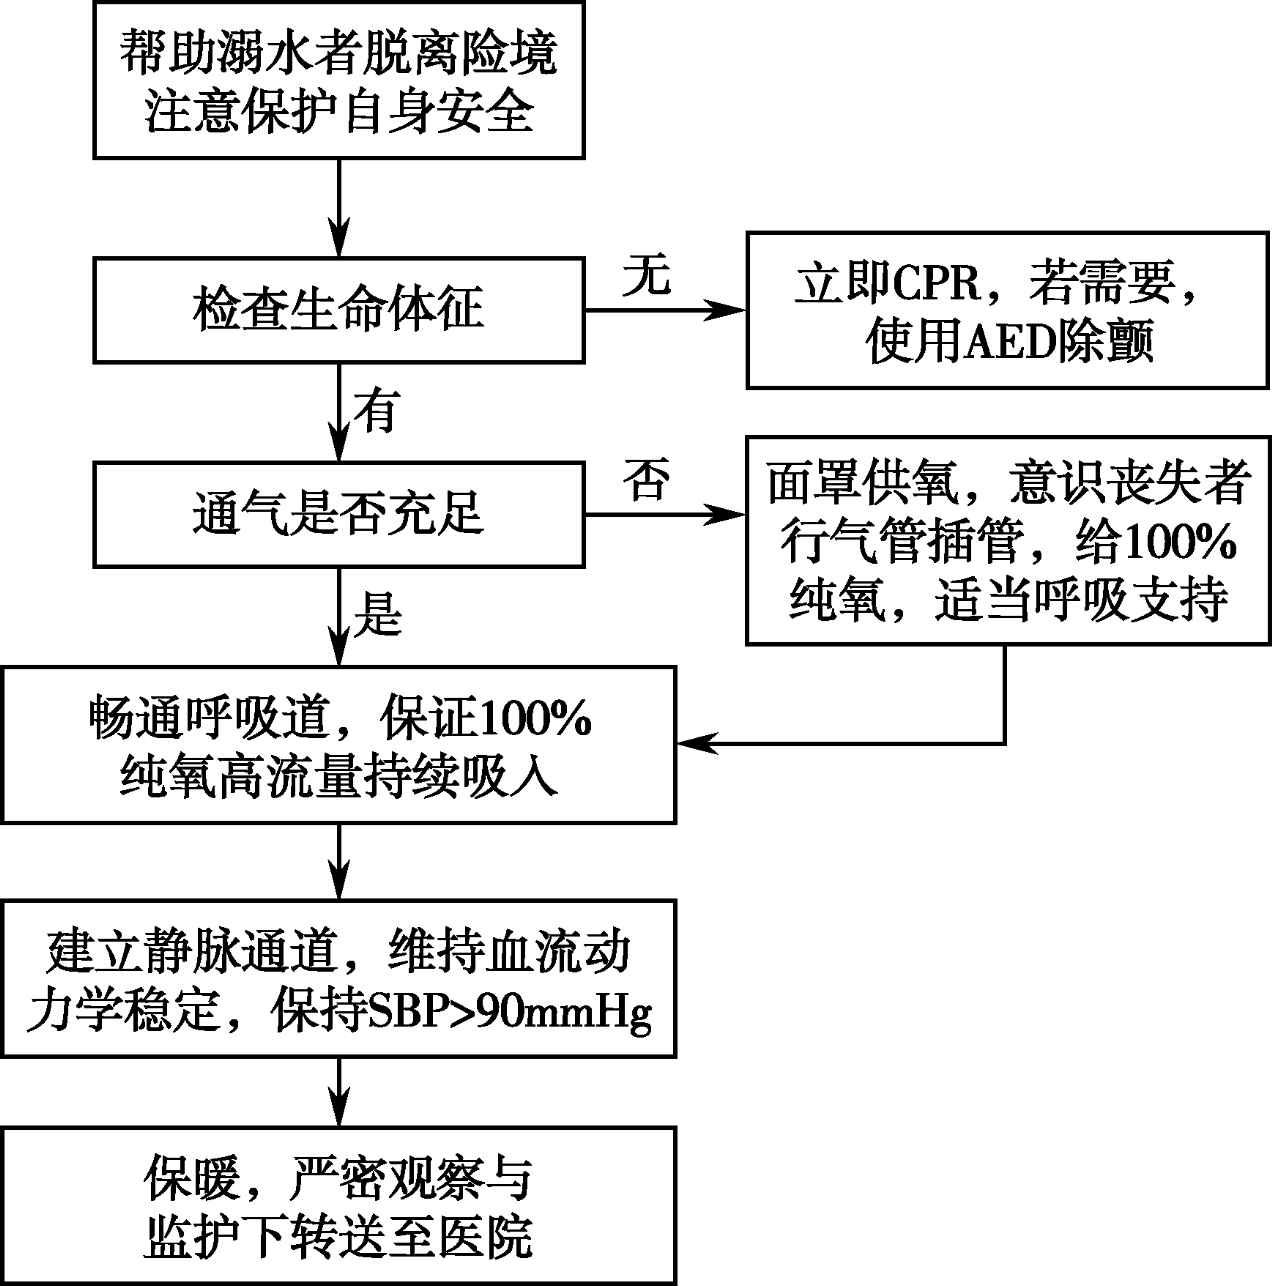
\includegraphics[width=2.89583in,height=2.91667in]{./images/Image00504.jpg}
 \captionsetup{justification=centering}
 \caption{淹溺的现场与院前急救要点}
 \label{fig132-1}
  \end{figure} 

\subsubsection{淹溺的院内急诊处理}

即使现场评估无任何异常,所有患者都应该转运到医院急诊进行进一步的观察、评估和处理。院内早期处理的重点是迅速复苏和防治呼吸衰竭;重视相关外伤的早期发现和恰当处理;保持供氧。具体措施主要包括:①继续CPR;②维持水、电解质和酸碱平衡;③防治感染;④头部、颈部与胸部CT或X线检查;⑤防治脑水肿与脑功能衰竭、ARDS、急性肾功能衰竭、急性心力衰竭、心律失常和DIC等,参见有关章节。

\protect\hypertarget{text00361.html}{}{}

\chapter{电 击 伤}

一定量电流或电能(静电)通过人体,引起不同程度的组织损伤或器官功能障碍,甚至死亡,称电击伤(electrical
injuries)。工业用电、家庭用电、雷电和生物电都可引起电击伤。由电源直接接触体表而发生的电击最常见,在高电压或超高电压的电场下,虽未直接接触电源,也会因电流经过空气时产生电弧,电弧长度可以从几厘米到1m以上,长短取决于电压的高低。这样人只要靠近高压线就可能受到损害。电流通过心、脑、延髓、脊髓等重要组织和脏器时常为致命性电击伤。低压电流可使心跳停止(或发生心室颤动),继之呼吸停止。高压电流由于对中枢神经系统强烈刺激,先使呼吸停止,再随之心跳停止。因此提高人们对电性能的认识,加强电站及供电系统的管理,严格遵守操作规程,是杜绝电击伤的必要前提;对触电者立即进行正确、有效的救治,是拯救患者生命,减少伤残的重要保证。

\subsection{病因与发病机制}

\subsubsection{病因}

电击伤的病因是电,这电可以是电流或静电的电能量。其原因包括:①生活中直接或间接接触漏电或工作中违反用电操作规程触电;②高温高湿场所,本来不漏电的电器绝缘性能降低后而发生漏电:身体受潮或出汗后电阻降低,本来不会触电的情况在此时因电流容易通过而发生触电;③旷野树下躲避雷雨,在雷雨的超高压电场中,电流或静电电荷经过空气或其他介质后电击人体;④抢救触电者时,营救者用手直接触拉等而导致电击伤;⑤意外情况,如风暴、地震、火灾等使电线断裂,带电的电线落在人体上,或由于某种原因误碰电源而致触电;⑥有些动物有发电器官,如:电鳗,放电时能引起剧痛,有时会使人晕厥,能造成淹溺事故。

常见的触电方式有三种:①单相触电:人体接触一根负载电线(火线),电流通过人体,并通过肢体与地面直接接触,大地成为回路,形成电流环形通路。②双相触电:人体不同部位同时接触同一线路上的两根有负载的电线,其一是火线,另一是零线(回路),电流从火线通过人体传导,由零线回流,形成环路。③跨步压触电:当一根电线落在地上,则以此电线落地点为圆心,在20m之内的地上有许多同心圆,这些不同直径的圆周内的电压各不相同,离电线落地点越近的圆周电压越高,越远则越低,这种电压称跨步电压。当人走入此电场感应区域,前脚跨出着地,后脚尚未离地,这时两脚分别接触在两个不同电位差的带电点上,存在电位差,即会使电流自前脚流入,经躯干再自后脚回流大地,形成环形通路。因其发生与跨步有关,故称为跨步压触电。此型触电,离电流落地点越近,电压越高,危险越大;跨步幅度越大,电位差越大,危险亦越大。

\subsubsection{发病机制}

低压和高压电流都可使细胞膜内外的离子水平发生变化,并发生电泳、电渗等反应,从而可导致器官的生物电节律周期发生障碍。接触中枢神经系统的电流即使仅有几十毫安,已可引起神经传导阻断,如累及脑干,呼吸迅速停止。较强的电流还可使呼吸肌强直性痉挛并直接引起胸腔压塞和窒息。断开连接后,肌肉强直性痉挛。电流穿过人体时,由于Joule效应可产生烧伤。另外,电闪和电弧可引起烧伤。这种烧伤,电流并不穿过身体,电能转化为热能在体外完成。高压电下,电弧能达2500度,造成Ⅲ度烧伤。这类烧伤与传统的热力烧伤没有任何区别。严重性在于电弧能造成角膜烧伤和白内障,有时要几个月后才会显现出来。

电击损伤对人体危害程度取决于电流强度、电压高低、电阻、径路、接触时间以及电流种类等。

\paragraph{电流强度}

是人体触电后致命因素。不同的电流量对人体产生不同的症状,一般2mA以下的少量电流,手指接触时仅产生麻刺感觉;当电流量增至10~20mA时,手指肌肉产生持续的收缩,不能自主松开电源,导致电流通过心脏时间较长,可致心肌细胞去极化,心肌收缩,并可引起剧痛和呼吸困难;如电流进一步增强至50~80mA,则可引起呼吸麻痹和心室纤维颤动;90~100mA,50~60周率的交流电即可引起呼吸麻痹,持续3秒心跳亦即停止而致死;220~250mA的直流电通过胸腔即可致死。2A以上,在电流通过的路径上产生神经抑制作用。

\paragraph{电压高低}

电压越高,电能越大,致伤的机会也越大。低电压强电流造成局部烧伤。一般认为,电器设备的电压在250V(伏)以上的称高压设备,36~250V的称低压设备,<
36V的称特低压设备。12V以下是绝对安全电压,36V以下是安全电压;220V电流可造成心室纤维颤动而致死;1000V以上电流可使呼吸中枢麻痹,呼吸停止,继而心跳停止而致死;220~1000V之间的致死原因则两者兼有。高电压还可使脑组织点状出血、水肿软化等。

\paragraph{电阻}

人体可以看作是一个由各种电阻不同的组织组成的导体,外面是一层导电能力很差的皮肤,皮肤里面有导电能力很强的体液。电流量=电压/电阻,在潮湿条件下,电阻降低,接触12V电流也有危险,20~40V电流作用于心脏也可致死。另外,电流接触人体后,在体内的线路不是按着直线进行,而是选择电阻小的组织前进,路线短则电阻小,如两指之间或嘴。血管、淋巴管是人体最好的导电体,肌腱、肌肉、神经次之,脂肪、皮肤更次之,骨骼的电阻最大,手掌、足跟及无发头皮等致密组织电阻亦最大。同样强度的电流由足跟进入,在局部皮肤可能造成一个不大的黄斑,流过肌肉、肌腱等组织,则造成局部重度电灼伤或炭化。通过人体的电流强度主要取决于人体的皮肤电阻与电源电流。冬季及皮肤干燥时,皮肤电阻可达到3万~100万Ω(欧姆);潮湿的皮肤可降至1000~5000Ω;皮肤裂开或破损时,电阻可降至300~500Ω。即在同样的电流电击下,后者较前者所通过的电流可大至数百至上千倍。

\paragraph{电流作用的时间}

时间越长,损伤越严重。当屈肌猛烈抽搐时,造成抓住导体紧紧不放的反应,可能延长接触时间。相反,如果肌抽搐作用在伸肌上,触电人失去知觉或被人看见断电了,则会远远弹开导体。高压电流通过人体时间<
0.1秒,不致引起死亡;超过1秒,可能导致死亡。

\paragraph{电流通过人体的径路}

凡电流通过心、脑等重要脏器往往有生命危险。穿胸电流(如手→手通路)较肢体电流(手→足,足→足)通路更易致死,主要原因为电流直接影响或冠脉痉挛,导致心肌损伤。

\paragraph{电流种类}

直流电、交流电、冲击电流和静电电荷对人体都有伤害作用。但人体对交流电的耐力要比直流电差得多,其中以低频(15~150Hz)的危险性为大。低频中又以50~60Hz的交流电危险性更大。低频交流电频率的改变,使其很容易作用于心电周期,引发室颤,类似于RonT现象。若频率超过2000Hz则危险性反而减少,如高频治疗机频率高达10万Hz,对人体毫无危害。

冲击电流和静电电荷对人体都能造成损害。雷电和静电都能产生冲击电流。静电为有限的电荷,往往在摩擦或电容器充电后发生。闪电为一种静电放电,其中电能量在1/2秒的时间内,以100亿伏的静电压放电,峰值电流可达200
000mA,这样高的电压电流的放电,可击毙在电路中的任何物体。由于所产生的高热和机械暴力,使击中者炭化,组织撕裂,并立即死亡,其死亡原因除严重的并发症外,一般认为系电击休克,心室纤维颤动和呼吸麻痹所致。

\subsection{诊断}

\subsubsection{病史}

有明确的触电或被雷、电击伤史。

\subsubsection{临床表现特点}

\paragraph{全身表现}

轻度电击者头晕、心悸、面色苍白、口唇发绀、四肢乏力、精神紧张,因惊恐而晕倒,并可能有肌肉疼痛,稍事休息即可完全恢复。中度电击者表现为惊恐,面色苍白,表情呆愣,触电肢体麻木感,部分患者甚至昏倒,暂时意识丧失,但瞳孔、血压无明显变化,患者呼吸浅而速,可出现偶发或频发期前收缩,心动过速。此时如及时处理,大多数患者可得以恢复。重度电击患者立即昏迷,抽搐;由低电压电流引起室颤时,皮肤苍白,听不到心音,触不到脉搏,开始时尚有呼吸,数分钟后呼吸即停止;高压电流引起呼吸中枢麻痹时,患者昏迷,呼吸停止,但心搏仍存在,血压下降,皮色青紫;如电压高,电流强,心脏与呼吸中枢同时受累,多立即死亡;也有电击后呈极微弱的心跳和呼吸的“假死状态”(即人体主要生理功能如心跳呼吸等,处于极微弱情况下的一种状态,外表看来似乎已经死亡),假死并非由室颤引起,主要由于延髓受抑制或呼吸肌痉挛所致。此外由于肢体的急剧抽搐动作可引起骨折。跌落或因猛烈抛出也可造成骨折,如有脊椎骨折甚至可能造成脊髓损伤。

受电击的肌肉与肾脏组织发生细胞溶解坏死后可产生大量肌红蛋白尿,溶血后血红蛋白尿可损伤肾小管,以及脱水和血容量不足等多种原因可共同促使患者发生急性肾功能衰竭。

\paragraph{局部表现(电热灼伤)}

因电压高低不同可造成局部不同程度的烧伤,一般低电压电流的烧伤面小,直径一般为0.5~2cm、呈圆形、椭圆形或蚕豆状,边缘规则整齐,与健康皮肤分界清楚,一般无痛,焦黄色、褐色或灰色干燥伤面,偶可见水疱形成。此类烧伤多见于电流进出口处,如手、臂或脚。在那些吮吸电源插座的孩子身上,嘴巴的电热烧伤,加上通过口水传播的电弧烧伤。严重的嘴唇和舌头烧伤造成大量坏死,有可能引起小口的并发症。

高压电流烧伤,由于电离子有较强大的穿透能力,因而烧伤的面积较大,损伤的深度也大,甚至深达肌肉和骨骼。轻者仅表现为皮肤干燥烧焦的创面,面积较大,损伤较深,可达真皮层或皮下组织;较重者可有大片焦痂,组织坏死,以后脱落,感染和渗出,伤口愈合较为缓慢,形成慢性皮肤溃疡。少数患者体表皮肤烧伤并不严重,甚至无明显皮肤改变,但电流更多地通过血管、淋巴管、肌肉、神经等,造成沿着其走向的灼伤,受伤当时可能表现不明显,早期常难以从外表确定损伤范围和程度,24~48小时后周围组织开始发红、肿胀、炎症反应;随病程进展,由于肌肉、神经或血管的凝固或断裂,可在一周或数周后逐渐表现坏死、感染、出血等,甚至发生脓毒症,后果严重。腹部电热灼伤可导致胆囊坏死、肠穿孔、胰腺炎、肠麻痹、肝脏损害、肾损伤,或因血浆肌红蛋白增高导致急性肾功能衰竭等。临床上对深部组织电灼的程度估计不足是诊断普遍存在的问题。

\paragraph{并发症}

电击伤极易并发急性肾功能衰竭。电流损害脊髓可致肢体瘫痪,血管损伤可致继发性出血或血供障碍,局部组织灼伤可致感染。触电常伴有外伤,如触电而从高处跌下,可伴有颅脑损伤,胸、腹部外伤或肢体骨折等;电击时因肌肉剧烈收缩的机械暴力,可致关节脱位和骨折。

\paragraph{后遗症}

①心血管后遗症,冠状动脉血栓的恶化或梗死后遗症,心前区疼痛,心脏节律异常的持续,心功能不全,肾功能的受损及血栓的后遗症。②中枢神经系统的后遗症如周围神经病变,上行性或横断性脊髓病变,侧索硬化症,瘫痪,大脑皮质萎缩,继发性癫痫,锥体外系症状。其中感觉神经后遗症,可以是视力方面的问题:枕叶梗死造成的同侧偏盲,视神经萎缩,电击伤性白内障,视觉精确度减弱,视网膜脱落加重,视网膜损伤,或者伴有耳聋和头晕的鼓膜外伤和内耳损伤造成的听觉问题。③功能后遗症来自于弯曲褶皱,异常的瘢痕,肌腱的损伤,甚至是截肢造成的粘连的挛缩。④心理后遗症,症状多样,近似于颅外伤的主观病症,消极,失眠,性格不稳定。

\paragraph{闪电损伤}

闪电击伤是遭受短暂的、非常强大的电流冲击引起的损伤。暴露的时间非常短暂,损伤常常局限在皮肤外层。闪电可以引起心脏和大脑的短路,使受害者立即死亡。双下肢常有暂时性瘫痪、呈蓝色、麻木(闪电性瘫痪)。皮肤可能有羽毛状或分支状的较小烧伤,由成簇的小点组成,像香烟头的烧伤或汗水蒸发后留下的条纹。皮肤血管收缩呈网状图案,为闪电损伤特征。

\subsubsection{实验室检查}

1.心肌和血管伤势评估
①反复心电图检查可见心动过缓,心动过速,ST段下移,T波倒置以及急性心肌梗死样变化。重症者出现心室颤动,心搏骤停。②动态心电监护。③CK-MB、肌红蛋白、肌钙蛋白定量。④超声波检测。⑤冠状动脉造影。⑥动脉、静脉造影术。

2.肌肉和肾伤势评估 ①CK定量;②寻找肌红蛋白尿;③肾功能检查。

3.神经伤势评估 ①头部和脊椎X线片和CT;②肌电图。

4.寻找相关外伤
①骨骼X线片,特别是肩胛骨,寻找骨折和脱臼;②胸部X线片,寻找支气管,纵隔积气,气胸和吸入损伤;③腹部平片,寻找空腔脏器穿孔造成的气腹。

5.寻找感觉损伤 ①眼科检查;②鼓膜和内耳检查。

6.触电的孕妇 ,必须对母体胚胎进行检查,如胎儿超声检查。

\subsection{治疗}

\subsubsection{脱离电源}

应争分夺秒,首要任务是迅速切断电源。按当时的具体环境和条件采用最快、最安全的办法切断电源或使患者脱离电源,一般有下述几种方法:

\paragraph{关闭电掣}

若电掣就在附近,立即关闭电掣是最简单、安全而有效的行动。并尽可能把保险盒打开,总电闸扳开,并派人守护总电掣闸,以防止忙乱中第三者重新合上电闸,导致其他人触电。这是一种十分重要而简便易行的安全措施。

\paragraph{斩断电线}

若在野外或远离电掣的地方,尤其是下雨时,不便接近触电者或挑开电源线者用之;或高压输电线断落,可能附近电场效应而会产生跨步电压者,应于20m以外斩断输电线(注意:斩断端的电线又可能触地形成新的中心,形成跨步电压,导致救护者触电)。所用的利器因地制宜选用,如绝缘钳子、干燥锄头、铲子、有干燥木柄的刀、斧等。

\paragraph{挑开电线}

对于高处垂落电源线触电,电掣不在附近,可用干燥木棒或竹竿挑开电源线。并注意挑开的电源线要放置好,避免他人触电。

\paragraph{拉开触电者}

如上述方法都不易用上,可用干木棒将触电者拨离触电处。如触电者趴在漏电的机器上,可用塑料绳、干绳子或衣服拧成带子,套在患者身上,将其拉出。

在使触电者离开电源的整个过程中,应注意以下几点:①必须严格保持自己与触电者的绝缘,包括不直接接触触电者,选用的器材必须是有可靠的绝缘性能。若对所用器材绝缘性能无把握,则要在操作时,脚下垫放干燥的木板、厚塑料块等绝缘物品,使自己与大地绝缘。②在下雨天气野外抢救触电者时,一切原先有绝缘性能的器材都因淋湿而失去绝缘性能,因此更需注意。③野外高压电线触电,注意跨步电压的可能性并予以防止,最好是选择20m以外进行切断电源;确实需要进出危险地带,需保持单脚着地的跨跳步进出,绝对不容许双脚同时着地。

\subsubsection{现场立即进行心肺复苏}

对呼吸微弱或不规则,甚至停止,但心搏尚在者,应立即口对口人工呼吸,和(或)胸外按压,并应同时准备行气管插管正压呼吸。对心搏停止者应立即行胸外按压。因为电击后存在“假死”状态,人工呼吸、胸外心脏按压必须坚持不懈进行,直至患者清醒或出现尸僵、尸斑为止。不可轻易放弃,可由几个人轮流操作。

\subsubsection{对症支持治疗}

主要是维持呼吸、血压稳定,积极防治脑水肿、急性肾功能衰竭等并发症,早期使用降温疗法,纠正水电解质及酸碱失调,防治继发感染。这些措施不单是在呼吸、心跳恢复后使用,而应在复苏开始时使用,并贯穿于抢救全过程。消毒纱布的包扎和有效的镇静止痛也很重要。尽量早期后送,搬动伤者时谨遵主干原则:头-颈-躯干,谨防加重脊髓外伤。后送至医院后,须多科进行会诊,根据临床检查选择住院科室。

\subsubsection{进一步治疗}

常规注射破伤风抗毒素。烧伤患者伤面周围皮肤用碘酒、酒精处理后,加盖消毒敷料包扎,减少污染。严重者须在烧伤科住院治疗,注意水、电解质和酸碱平衡紊乱的纠正,分期进行预防或治疗肾功能不全的血液透析和预防控制感染并发症。已有坏死肢体采用暴露疗法,伤后3~5天坏死分界线清楚后,进行坏死组织清创术,并注意创口继发性出血,并给予相应处理。择期行植皮治疗。针对压迫性筋膜下水肿作筋膜切开减张术。对于严重损伤而不能保留的肢体,须行截肢,以免坏死物质吸收而引起急性肾功能不全。如有骨折、颅脑外伤等,则在复苏的基础上同时进行积极处理。选用有效抗生素防治继发感染,特别要注意厌氧菌感染的防治。

\subsubsection{其他}

电击伤后引起机体严重缺氧者较多见,一般氧疗不能奏效者可用高压氧治疗,以提高氧含量,增加氧分压和血氧的弥散,有效纠正缺氧。对神志清楚,伴有乏力、心慌、全身软弱的患者,一般卧床休息数天后即能恢复,必要时对症支持治疗。并应注意深部烧伤及可能的远期并发症。另外,进行早期的心理干预也很重要。

\protect\hypertarget{text00362.html}{}{}

\hypertarget{text00362.htmlux5cux23CHP15-5-4}{}
参 考 文 献

1. 张文武 .急诊内科学.第2版.北京:人民卫生出版社,2007:1425

2. Pierre Carli,Bruno Riou,Caroline
Télion,赵剡译.急诊医学---成人内-外科学.北京:科学出版社,2009:725

3. Mark H.
Beers.赵小文,译.默克家庭诊疗手册.第2版.北京:人民卫生出版社,2006:1368

\protect\hypertarget{text00363.html}{}{}

